\documentclass[12pt]{ctexart}

\title{机械设计基础课程设计报告}
\author{欧 宇恒}
\date{\today}
\usepackage{ctex}			%处理中文字体宏包
\usepackage{graphicx}		%处理图片宏包
\usepackage{amsmath}		%处理数学公式宏包	
\usepackage{setspace}		%处理行距宏包
\usepackage[left=1.91cm,right=1.91cm,top=2.54cm,bottom=2.54cm]{geometry}		%编辑页面格式
\usepackage{booktabs}		%处理三线表宏包
\usepackage{color}			%处理颜色宏包
\usepackage{multirow}       %处理合并单元格宏包
\usepackage{longtable}


\begin{document}	
	\ctexset{
		section={
			name={\S},
			nameformat={\zihao{2}},
			titleformat={\centering\heiti\zihao{2}},
		},
		subsection={
			name={},
			nameformat={\zihao{4}},
			titleformat={\zihao{4}},
		},
	}

    
\begin{titlepage}

    \begin{center}
    % Upper part of the page
    
\includegraphics[width=0.4\textwidth]{CSU.png}\\[1cm]    
    \textsc{\LARGE Central South University}\\[1.5cm]
    \textsc{\Large Final Week Project}\\[1.5cm]
    % Title
    \textsc{\huge \bfseries 机械设计基础课程设计说明书}\\[1.5cm]
    % Author and supervisor
    \begin{minipage}{0.4\textwidth}
    \begin{flushleft} \large
    \emph{Author:}\\
    欧宇恒\\
    \emph{ID:}\\
    8212210728\\
    \emph{class:}\\
    交设 2105 班\\
    \end{flushleft}
    \end{minipage}
    \begin{minipage}{0.4\textwidth}
    \begin{flushright} \large
    \emph{Supervisor:} \\
    周英
    \end{flushright}
    \end{minipage}
    
    \vfill
    
    % Bottom of the page
    {\large \today}
    
    \end{center}
    
    \end{titlepage}
%%封面


%%封面 end

\newpage

\tableofcontents

\newpage

\section{运动参数、动力参数的确定}

\subsection{电动机型号选择}

根据所给题目要求,本小组已知参数为输送带的牵引力$F=3.5\text{kN}$,输送带的速度$v=1.8\text{m/s}$,输送带滚筒直径$D=350\text{mm}$,由此可以计算出工作机所需功率 (kW):

$$P_W=Fv=33.5\times 1.8=6.3\text{kW}$$

其次,通过查表 [2]P7 表 2-4,可得齿轮、轴承、联轴器的传动效率,依据本题具体情况,取各传动效率如下:

\begin{table}[h]
    \setlength{\belowcaptionskip}{0.3cm}
    \centering
    
    \caption{各传动构件传动效率}
    \begin{tabular}{c c}
        \toprule
        传动构建 & 效率 \\
        \midrule
        V 带 & 0.96\\
        滚动轴承 & 0.98\\
        齿轮 & 0.96\\
        联轴器 & 0.99\\
        \bottomrule
    \end{tabular}
    
\end{table}

故可得总传动效率为:

$$\eta_\text{总} = \eta_\text{带}\eta^3_{\text{轴承}}\eta_{\text{齿轮}}\eta_{\text{联轴器}}=0.96\times 0.98^3\times 0.96\times 0.99 = 0.86$$

由此可以计算出电动机需要提供的输入功率:

$$P_d = \frac{P_W}{\eta_\text{总}} = \frac{6.3}{0.86} = 7.33\text{kW}$$

本小组选取电动机转速为 $1000\text{r/min}$,考虑到选择的电动机功率$P_d'>P_d$,故通过查阅 [2]P196 表 20-1 得到应选取电动机型号为 Y160M-6,该型号电动机的额定满载转速为$n_m=970\text{r/min}$。

对于输出卷筒而言,计算其工作转速为:

$$n_W = \frac{60000v}{\pi D} = \frac{60000\times 1.8}{\pi \times 350} = 98\text{r/min}$$

故可得减速器的总传动比为:

$$i_\text{总} = \frac{n_m}{n_W}=\frac{970}{98}=9.87$$

本课设中,选取齿轮传动比为 3.06,则此时带传动比为 3.23,均在要求范围之内。选取小齿轮齿数为 29,大齿轮齿数为 89,满足齿轮传动比要求,并且齿数互质,有较好的传动性能。

\subsection{运动参数与动力参数计算}

\begin{figure}[htbp]
    \centering
    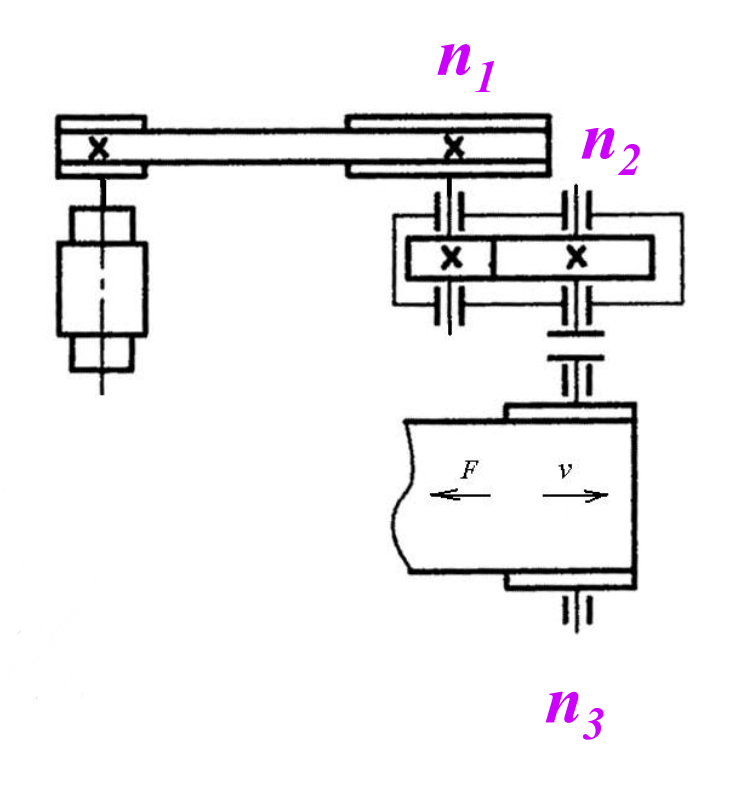
\includegraphics[scale=0.2]{dynamic_argument.png}
    \quad
    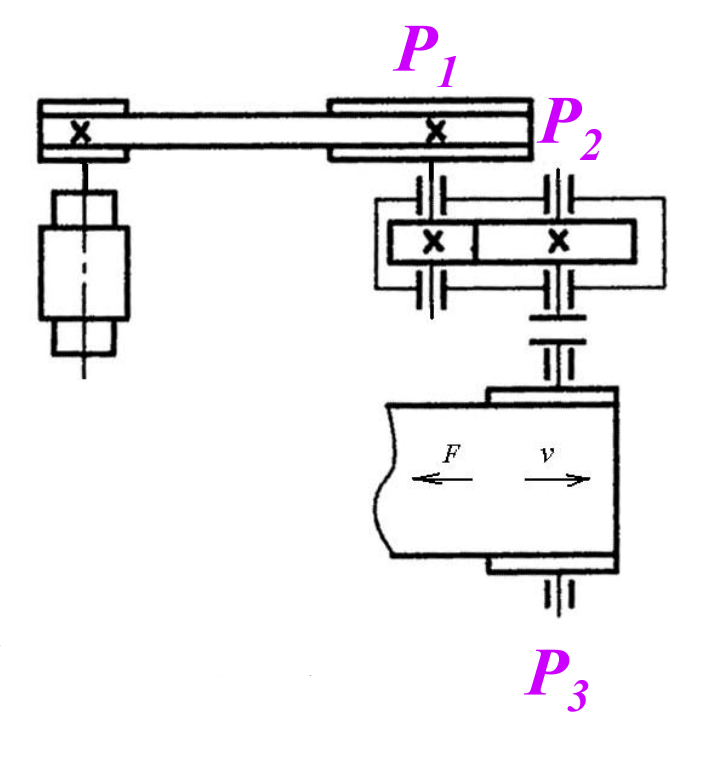
\includegraphics[scale=0.2]{P.png}
    \caption{各机构运动转速与工作功率示意图}\label{figure1}
\end{figure}

各构件工作转速和工作功率如图\ref{figure1}所示,通过传动比计算可得:

$$n_1=\frac{n_m}{i_\text{带}}=\frac{970}{3.23}=301\text{r/min}$$

$$n_2=\frac{n_1}{i_{\text{齿轮}}}=n_3=n_W=98\text{r/min}$$

各个轴的功率计算:

$$P_1 = P_d\eta_{\text{带}}=7.33\times 0.96 = 7.04 kW$$

$$P_2 = P_1 \eta_{\text{轴承}}\eta_{\text{齿轮}}=7.04\times 0.98\times 0.96 = 6.62 kW$$

$$P_3 = P_2 \eta_{\text{轴承}}\eta_{\text{联轴器}}=6.62\times 0.98\times 0.99=6.43 kW$$

各轴上都是以该轴上的最大功率(即:输入功率)作为设计所用,故可以算出各轴上的传动力矩:

$$T_1 = 9550\frac{P_1}{n_1} = 9.55\times 10^6\times \frac{7.04}{301}=223672.1\text{N·mm}$$

$$T_2 = 9550\frac{P_2}{n_2} = 9.55\times 10^6\times \frac{6.62}{98}=643917.9\text{N·mm}$$

$$T_3 = 9550\frac{P_3}{n_3} = 9.55\times 10^6\times \frac{6.43}{98}=624729.2\text{N·mm}$$

将以上结果汇总后,得到表\ref{table1},列出了各个轴的输入功率、工作转速与传动扭矩,至此,课程设计的运动参数和动力参数确定完毕。

\begin{table}[h]
    \centering
    \setlength{\belowcaptionskip}{0.3cm}
    \caption{运动参数与动力参数汇总表}\label{table1}
    \begin{tabular}{c c c c c}
        \toprule
        轴号 & 功率$P/\text{kW}$ & 转速$N/\text{(r/min)}$ & 扭矩$T/\text{N·mm}$ & 传动比$i$ \\
        \midrule
        电机轴 & 7.33 & 970 & 72264.95 & \multirow{ 2}{*}{$i_{\text{带}}=3.23$}\\
        I & 7.04 & 301 & 223672.1 & \\
        II & 6.62 & 98 & 643917.9 & \multirow{ 2}{*}{$i_{\text{齿轮}}=3.06$}\\
        III & 6.43 & 98 & 624729.2 & \\
        \bottomrule
    \end{tabular}
    
\end{table}
    


\section{齿轮设计计算方法}

本课程设计选用闭式齿轮进行齿轮设计,
设齿轮传动比$i_{12}=3.1$,
高速轴转速$n_1=301 \text{r/min}$,
传动功率$P=7\text{kW}$,
考虑到该课程设计中的齿轮需有较好的接触疲劳强度,
故采用软齿面设计,
通过参考文献 [1]P179 提供的方法对齿轮进行设计。

\subsection{选择材料及确定许用应力}

小齿轮采用 45 号调质钢作为材料,
并作调质热处理,
齿面硬度为 $197\sim 286\text{HBS}$,
接触疲劳极限为$\sigma_{Hlim}=550\sim 620\text{MPa}$,
弯曲疲劳极限$\sigma_{FE}=410\sim 480\text{MPa}$,
此时相应的疲劳强度取均值得,
$\sigma_{Hlim1} = 585\text{MPa}$,
$\sigma_{FE1}=445\text{MPa}$,
由于大小齿轮均为软齿面,考虑到小齿轮齿根较薄时,弯曲强度较低,受载次数多,故对大齿轮做正火热处理,使得小齿轮的弯曲疲劳极限稍高于大齿轮,大、小齿轮的弯曲强度近乎相近

故此时对大齿轮而言,
齿面硬度为 $156\sim 217\text{HBS}$,
接触疲劳极限为$\sigma_{Hlim}=350\sim 400\text{MPa}$,
弯曲疲劳极限$\sigma_{FE}=280\sim 340\text{MPa}$,
此时相应的疲劳强度取均值得,
$\sigma_{Hlim2} = 375\text{MPa}$,
$\sigma_{FE2}= 310\text{MPa}$
(由 [1]P171 表 11-1 查得)。

又由 [1]P176 表 11-5,取一般可靠度,
在失效概率$\le 1/100$时,
最小安全系数取:$S_H=1$, $S_F=1.25$。

综上所述,齿轮材料参数的设计见表\ref{label_1}所示。

\begin{table}[htbp]
    \centering
    \setlength{\belowcaptionskip}{0.3cm}
    \caption{齿轮材料设计参数}
    \begin{tabular}{c c c c}
        \toprule
        \textbf{齿轮材料参数} & \textbf{硬度/HBS} & \textbf{接触疲劳强度} & \textbf{弯曲疲劳强度} \\
        \midrule
        小齿轮 & $197\sim 286 HBS$ &  $\sigma_{Hlim1} = 550\sim 620\text{MPa}$ & $\sigma_{Flim1} = 410\sim 480\text{MPa}$ \\
        大齿轮 & $156\sim 217 HBS$ & $\sigma_{Hlim2} = 350\sim 400\text{MPa}$ & $\sigma_{Flim2} = 280\sim 340\text{MPa}$ \\
        \bottomrule
    \end{tabular}
    
    \label{label_1}
\end{table}


\begin{table}[htbp]
	\centering
    \setlength{\belowcaptionskip}{0.3cm}
	\caption{最小安全系数表}
    \begin{tabular}{cc}
		\toprule
		接触疲劳最小安全系数$S_H$ & 弯曲疲劳最小安全系数$S_F$ \\
		\midrule
		 1 & 1.25 \\
		\bottomrule
	\end{tabular}

\end{table}


接下来可计算许用应力:

$$[\sigma_{H1}]=\frac{\sigma_{Hlim1}}{S_H}=\frac{585}{1}\text{MPa}=585\text{MPa}$$

$$[\sigma_{H2}]=\frac{\sigma_{Hlim2}}{S_H}=\frac{375}{1}\text{MPa}=375\text{MPa}$$

$$[\sigma_{F1}]=\frac{\sigma_{FE1}}{S_F}=\frac{445}{1.25}\text{MPa}=356\text{MPa}$$

$$[\sigma_{F2}]=\frac{\sigma_{FE2}}{S_F}=\frac{310}{1.25}\text{MPa}=248\text{MPa}$$

\subsection{按齿面接触强度设计}

本课程设计中齿轮按照 8 级精度设计,取载荷系数$K=1.2$(由 [1]P174 表 11-3 查得),齿宽系数$\phi_d=1$(由 [1]P179 表 11-6 查得),小齿轮上的转矩
$$T_1 = 2.18 \times 10^5 \text{N·m}$$
取弹性系数$Z_E = 189.8 \sqrt{\text{MPa}}$(由 [1]P175 表 11-4 查得),$u=i_{12}=3.06$,则:

\begin{align*}
    d_1 & \ge 2.32\sqrt[3]{\frac{KT_1}{\phi_d}\frac{u+1}{u}\left(\frac{Z_E}{[\sigma_{H}]}\right)^2}\\
    & = 2.32\sqrt[3]{\frac{1.2\times 2.18 \times 10^5}{1}\frac{3.06+1}{3.06}\left(\frac{189.8}{375}\right)^2} \\
    & =103.69 mm 
\end{align*}

齿数取$z_1=29$,则$z_2=3.06\times 29\approx 89$,故:
模数

$$m=\frac{d_1}{z_1}=\frac{103.69}{29}\text{mm}=3.57\text{mm}$$

按 [1]P58 表 4-1 取$m=4\text{mm}$,实际的$d_1 = zm=29\times 4=116\text{mm}, d_2=89\times 4=356\text{mm}$,则:

中心距$$a = \frac{d_1+d_2}{2} = 236\text{mm}$$


大齿轮齿宽

$$b_2=\phi_dd_1=1\times 116\text{mm}=116\text{mm}$$
圆整后取$b_2=120\text{mm}$。

小齿轮齿宽应设计的较大齿轮宽$5\sim 10 \text{mm}$,保证齿轮有足够的啮合宽度,故设:

$$b_1 = b_2 + 5 = 125 \text{mm}$$


\subsection{验算齿轮弯曲强度}

齿形系数由 [1]P177 图 11-8 得,$Y_{Fa1}=2.62,Y_{Fa2}=2.24$,由 [1]P178 图 11-9 得,$Y_{Sa1}=1.63,Y_{Sa2}=1.78$,由 [1]P177 式 11-5,

$$\sigma_{F1}=\frac{2KT_1Y_{Fa}Y_{Sa}}{bd_1m}=\frac{2\times 1.2 \times 2.18\times 10^5\times 2.62\times 2.24}{116\times 116\times 4} = 41.69 \le [\sigma_{F1}]=356\text{MPa}$$

$$\sigma_{F2}=\sigma_{F1}\frac{Y_{Fa2}Y_{Sa2}}{Y_{Fa1}Y_{Sa1}}=41.69\times \frac{2.24\times 1.78}{2.62\times 1.63}=38.92\text{MPa}\le [\sigma_{F2}]=248\text{MPa}$$

\subsection{齿轮的圆周速度}

$$v = \frac{\pi d_1n_1}{60\times 1 000}=\frac{\pi \times 116\times 301}{60\times 1000}\text{m/s} = 1.82\text{m/s}$$

对照 [1]P172 表 11-2 可知选用 8 级精度是合适的,至此齿轮设计完毕。

\subsection{圆柱齿轮在装配图中的参数设计}

查 [2]P66 表 9-2,可得圆柱齿轮在装配图中的各项参数取值。本设计中采取模锻齿轮的腹板式结构,通过计算并取圆整后,圆柱齿轮上的设计如表\ref{table17}所示。

\begin{table}[htbp]
    \centering
    \setlength{\belowcaptionskip}{0.3cm}
    \caption{圆柱齿轮在装配图中的参数设计值}
    \begin{tabular}{c l c}
        \toprule
        参数 & 计算方法 & 尺寸值/mm \\
        \midrule
        $d$   & 轴孔直径 & 67 \\
        $d_a$ & 齿顶圆直径 & 364 \\
        $m$   & 模数      & 4 \\
        $d_f$ & 齿根圆直径 & 346 \\
        $B$   & 齿宽     & 116\\
        $n$   & $n=0.5m$ & 2 \\
        $d_1$ & $d_1=1.6d$ & 110 \\
        $D_0$ & $D_0=0.5(D_1+d_1)$ & 217 \\
        $\delta_0$ & $\delta _0=(2.5\sim 4)m\ge 10$ & 12 \\
        $D_1$ & $D_1=d_f-2\delta_0$ & 322 \\
        $d_0$ & $d_1=0.25(D_1-d_1)$ & 53 \\
        $r$   & $r=5$       & 5\\
        $C$   & $C=0.3B$    & 36\\
        $C_1$ & $C_1=(0.2\sim 0.3)B$ & 32\\
        \bottomrule
    \end{tabular}
    
    \label{table17}
\end{table}


\section{带传动设计计算方法}

本课程设计需要设计一 V 带传动,选用异步电动机为驱动,电动机型号选取为:Y160M-6,电动机满载转速为:$n_1 = 970\text{r/min}$,V 带大轮转速为$n_2=301\text{r/min}$,因此可以计算出传动比为:$i_{12}=n_1/n_2=3.22$,V 带输入功率为$P=7.5\text{kW}$,设计为两班制工作。

\subsection{求计算功率$P_c$}

考虑到本课程设计使用的 V 带,载荷平稳,用于小批量生产,为载荷变动很小的轻负荷输送机,由 [1]P222 表 13-9 查得,在两班制工作状态下,选取工作情况系数$K_A=1.2$,故计算功率$P_c=K_AP=9\text{kW}$。

\subsection{选 V 带型号}

本课程设计选用普通 V 带,根据$P_c=9\text{kW},n_1=970\text{r/min}$,由 [1]P223 图 13-15 查得此坐标点落在 B 型区域,故选用 B 型进行计算。

\subsection{求大、小带轮基准直径$d_2$、$d_1$}

由 [1]P223 图 13-15 得到,$d_1 = 125\sim 140\text{mm}$,因传动比不大,$d_1$可取较大值而不会使$d_2$过大,先取$d_1=140\text{mm}$,取弹性传动比$\varepsilon = 0.02$,由 [1]P215 式 13-8 得到:

$$d_2 = \frac{n_1}{n_2}d_1(1-\varepsilon)=\frac{970}{301}\times 140\times (1-0.02)\text{mm} = 442.14\text{mm}$$

由  [1]P224 表 13-10 查得,取$d_2=450\text{mm}$(虽使得$n_2$有所减小,但是误差在 5\%以内,允许)。

\subsection{验算带速}

$$v =\frac{\pi d_1n_1}{60\times 1000}=\frac{\pi \times 140 \times 970}{60\times 1000}\text{m/s}=7.11\text{m/s}$$带速在$5\sim 30$m/s 范围内,合适。

\subsection{求 V 带基准长度$L_d$与中心距$a$}

初步选取中心距$a_0=1.5(d_1+d_2)=1.5\times (140+450)=885\text{mm}$,取$a_0=900$

此时,由 [1]P209 式 13-2 带长

\begin{align*}
    L_0 & =2a_0+\frac{\pi}{2}(d_1+d_2)+\frac{(d_2-d_1)^2}{4a_0} \\
    & =\left[2\times 900 + \frac{\pi}{2}\times (140+450)+\frac{(450-140)^2}{4\times 900}\right]\\
    & =2753.46\text{mm}
\end{align*}

由 [1]P216 表 13-2 查得,B 型 V 带选用$L_d=2700\text{mm}$,带长修正系数$K_L=1.04$,再由 [1]P224 式 13-15 计算实际中心距:

$$a \approx a_0 + \frac{L_d-L_0}{2}=900 + \frac{2700-2753.46}{2}\text{mm}=873.27\text{mm}$$

\subsection{验算小带轮包角$\alpha_1$}

由 [1]P209 式 13-1 得到,

$$\alpha_1=180^\circ -\frac{d_2-d_1}{a}\times 57.3^\circ =159.66^\circ > 120^\circ $$
合适。

\subsection{求 V 带根数$z$}

由 [1]P222 表 13-8 查得,在包角$\alpha_1=159.66^\circ$时,包角修正系数$K_\alpha = 0.95$,由 [1]P219 表 13-4 查得,普通 V 带的基本额定功率$P_0 = 2.08\text{kW}$,此时传动比 由 [1]P215 式 13-8 得到:

$$i_{12}=\frac{d_2}{d_1(1-\varepsilon)}=\frac{450}{140\times (1-0.02)}=3.28$$误差在 5\%,可以允许。

又由 [1]P221 表 13-6 查得,额定功率增量$\Delta P_0=0.30\text{kW}$

可由 [1]P223 式 13-14 得:

$$z =\frac{P_c}{[P_0]} = \frac{P_c}{(P_0+\Delta P_0)K_\alpha K_L}=\frac{9}{(2.08+0.3)\times 0.95\times 1.04}=3.81$$取 4 根。

\subsection{求作用在带轮轴上的压力$F_Q$}

由 [1]P216 表 13-1 查得,单位长度质量$q=0.170\text{kg/m}$,故由 [1]P225 式 13-16 得单根 V 带的初拉力为:

\begin{align*}
    F_0 & = \frac{500P_c}{zv}\left(\frac{2.5}{K_\alpha}-1\right) + qv^2\\
    & = \left[\frac{500\times 9}{4\times 7.11}\times \left(\frac{2.5}{0.95}-1\right)+0.17\times 7.11^2\right]\text{N}\\
    & = 266.74\text{N}
\end{align*}

作用在轴上的压力:

$$F_Q = 2zF_0\sin \frac{\alpha_1}{2}=2\times 4\times 266.74\times sin(\frac{160^\circ}{2})\text{N}=2100.38\text{N}$$

至此 V 带设计完毕。

\section{轴的设计计算}

\subsection{初算轴的最小直径}

由于本课程设计中齿轮与轴的材料选取同一种材料,高速齿轮轴材料为 45 号调质钢,低速齿轮轴材料为 45 号钢采用正火处理,轴的最小直径估算公式为:

$$d_{min}=C\sqrt[3]{\frac{P}{n}}$$

其中,$P$为轴的输入功率,$n$为轴的转速,$C$由轴的材料和承载情况确定,依据 [1]P250 表 14-2,初步暂定$C=110$,则有

$$d_{min,1}=110\times \sqrt[3]{\frac{7.04}{301}} = 31.46\text{mm}$$

$$d_{min,2}=110\times \sqrt[3]{\frac{6.62}{98}} = 44.78\text{mm}$$

此时定出的轴径为最小直径,但是由于轴伸处需要切开键槽,需要额外加粗 5\%的轴径,加粗后的轴径为:

$$d_{min,1,plus} = d_{min,1}\times 105\% = 33.03\text{mm}$$

$$d_{min,2,plus} = d_{min,2}\times 105\% = 47.01\text{mm}$$

\begin{figure}[htbp]
    \centering
    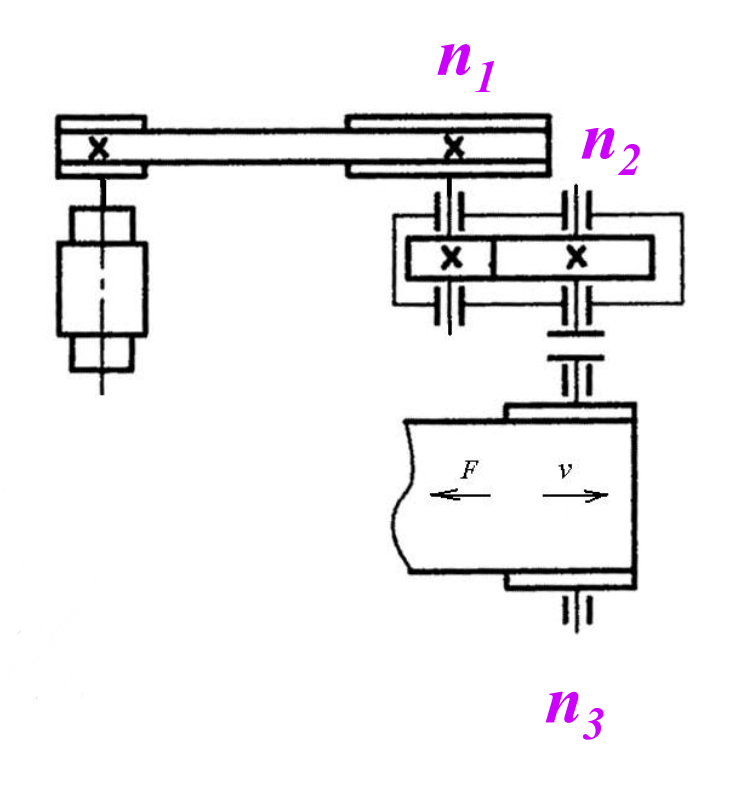
\includegraphics[scale=0.2]{dynamic_argument.png}
    \caption{轴连接示意图}\label{figure7}
\end{figure}

由图\ref{figure7}可以看出,高速轴和低速轴连接的为带轮和联轴器,需要根据标准选择基准直径。高速轴的轴伸连接 V 带轮,需要根据 V 带轮的标准直径选取,查 [3]P227 表 8-15,选取高速轴的基准直径为 $35\text{mm}$;低速轴的轴伸连接联轴器,根据联轴器的标准选取,查 [2]P162 表 17-2,选取低速轴的基准直径为 $50\text{mm}$。

\subsection{带轮的选择}

考虑到本设计选用 B 型带轮,依据大带轮基准直径,通过查 [2]P64 表 9-1,可得带轮的一系列参数如表\ref{table27}所示。

\begin{table}[htbp]
    \centering
    \setlength{\belowcaptionskip}{0.3cm}
    \caption{大带轮选用型号及参数}
    \begin{tabular}{c c}
        \toprule
        参数 & 尺寸值 \\
        \midrule
        V 带型号         & B 型 \\
        $d_d$           & 450 \\
        轮毂长度$l$     & 70 \\
        孔径$d$         & 35 \\
        \bottomrule
    \end{tabular}
    
    \label{table27}
\end{table}

\subsection{联轴器的选择}

本设计中低速轴与工作机轴相连接,可采用常见的凸缘联轴器,根据公称扭矩,查 [2]P162 表 17-2,主动端选择 J 型轴孔,从动端选择 J1 型轴孔,主从动端轴伸均选用 C 型键槽,因此可选用联轴器型号为:

$$ \text{YL11 联轴器} \frac{JC50\times 84}{J_1C55\times 84}GB5843-86 $$ 

可以得到联轴器各项参数如表\ref{table28}所示。

\begin{table}[htbp]
    \centering
    \setlength{\belowcaptionskip}{0.3cm}
    \caption{联轴器参数}
    \begin{tabular}{c c}
        \toprule
        参数 & 参数值 \\
        \midrule
        主动端轴孔长度   & 84 \\
        从动端轴孔长度   & 84 \\
        $L_0$           & 173 \\
        $D$             & 160 \\
        $D_1$          & 130 \\
        螺栓数量        & 4* (铰制孔连接)\\
        螺栓直径        & M12\\
        \bottomrule
    \end{tabular}

    \label{table28}
\end{table}

\subsection{确定各轴段直径}

接下来需要确定各轴段直径,各轴段序号标注如图\ref{figure8}所示:

\begin{figure}[htbp]
    \centering
    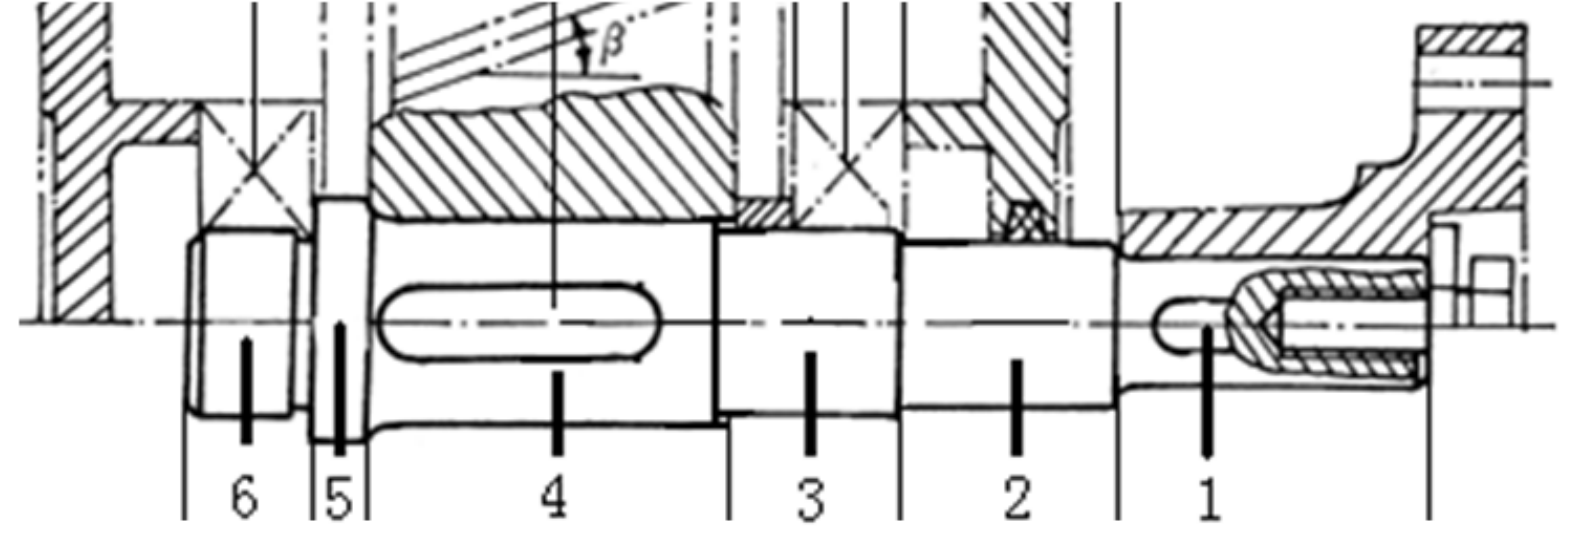
\includegraphics[scale=0.2]{roller.png}
    \caption{轴段序号标注示意图}\label{figure8}
\end{figure}

其中,轴段 1 的直径为前期计算已经确定的最小基准轴径;

轴段 2 则根据密封圈标准件的基准直径确定,且要求 D2 较 D1 大于 $6\sim 10 \text{mm}$ 通过查表 [2] P158 表 16-9 可得;

轴段 3 的直径较 D2 大于$1\sim 5\text{mm}$且需要为 5 的倍数,以此匹配轴承的需要;

轴段 4 的直径较 D3 大于$1\sim 5\text{mm}$,需要与大齿轮匹配,需要查 [2]P117 表 11-2 查出大齿轮的基准直径;

轴段 5 有定位要求,需要较 D4 大 $6 \sim 10 \text{mm}$;由于同一根轴上的两轴承内外径大小一致;

轴段 6 与轴段 3 直径相等,但同时需要满足轴承安装高度的要求(如表\ref{table10}所示),考虑到在高速轴中,轴承安装高度与 D5 矛盾,需要将 D5 设计成两段阶梯的轴肩,设计出的各轴段直径设计尺寸如表\ref{table9}所示。

查轴承的安装尺寸,查 [2]P144 表 15-3,得到高速轴与低速轴选用轴承与相关参数,汇总如表\ref{table10}所示,。
\begin{table}[htbp]
    \centering
    \setlength{\belowcaptionskip}{0.3cm}
    \caption{轴承选用型号及参数}
    \begin{tabular}{c c c}
        \toprule
        型号及参数 & 高速轴 & 低速轴\\
        \midrule
        轴承型号 & 6309(新标准) & 6313(新标准) \\
        内径$d$/mm & 45 & 65 \\
        外径$D$/mm & 100 & 140 \\
        安装尺寸/mm & 54 & 77 \\
        轴承宽度/mm & 25 & 33 \\
        径向基本额定动载荷$C_r$/kN & 40.8 & 72.2 \\

        \bottomrule
    \end{tabular}

    \label{table10}
\end{table}


\begin{table}[htbp]
    \centering
    \setlength{\belowcaptionskip}{0.3cm}
    \caption{各轴段直径设计尺寸}
    \begin{tabular}{c c c}
        \toprule
        直径 & 高速轴 & 低速轴\\
        \midrule
        D1/mm & 35 & 55 \\
        D2/mm & 42 & 60 \\
        D3/mm & 45 & 65 \\
        D4/mm & 50 & 67 \\
        D5/mm & 54(左),56(右) & 75 \\
        D6/mm & 45 & 65 \\
        \bottomrule
    \end{tabular}
    
    \label{table9}
\end{table}

\subsection{润滑方式选择}

\subsubsection{轴承的润滑方式选择}

本设计通过速度因数$dn$值对轴承润滑方式选择,根据 [1]P289 图 16-11 选择润滑方式。

通过计算,本设计中各个轴承的$dn$值如表\ref{table12}所示:

\begin{table}[htbp]
    \centering
    \setlength{\belowcaptionskip}{0.3cm}
    \caption{各轴承速度因数值}
    \begin{tabular}{c c c c}
        \toprule
        轴 & 轴承内径/mm & 转速/(r/min) & 速度因数/(r·mm/min)\\
        \midrule
        高速轴 & 45 & 301 & 13545 \\
        低速轴 & 65 & 98  & 6370  \\
        \bottomrule
    \end{tabular}
    
    \label{table12}
\end{table}

由于高速轴和低速轴的速度因数均$<(2\sim 3)\times 10^5 \text{mm·r/min}$,故均选用脂润滑。

\subsubsection{齿轮的润滑方式选择}

由于本设计中齿轮的轮系速度$v<12m/s$,故齿轮的润滑方式选择油润滑。

\subsection{轴段长度确定}

本项目中采取脂润滑的轴承,参考 [2]P26 图 4-3 进行设计,如图\ref{figure9}所示。各个轴段长度需要根据画图确定,各段长度确定方法确定如下。

\begin{figure}
    \centering
    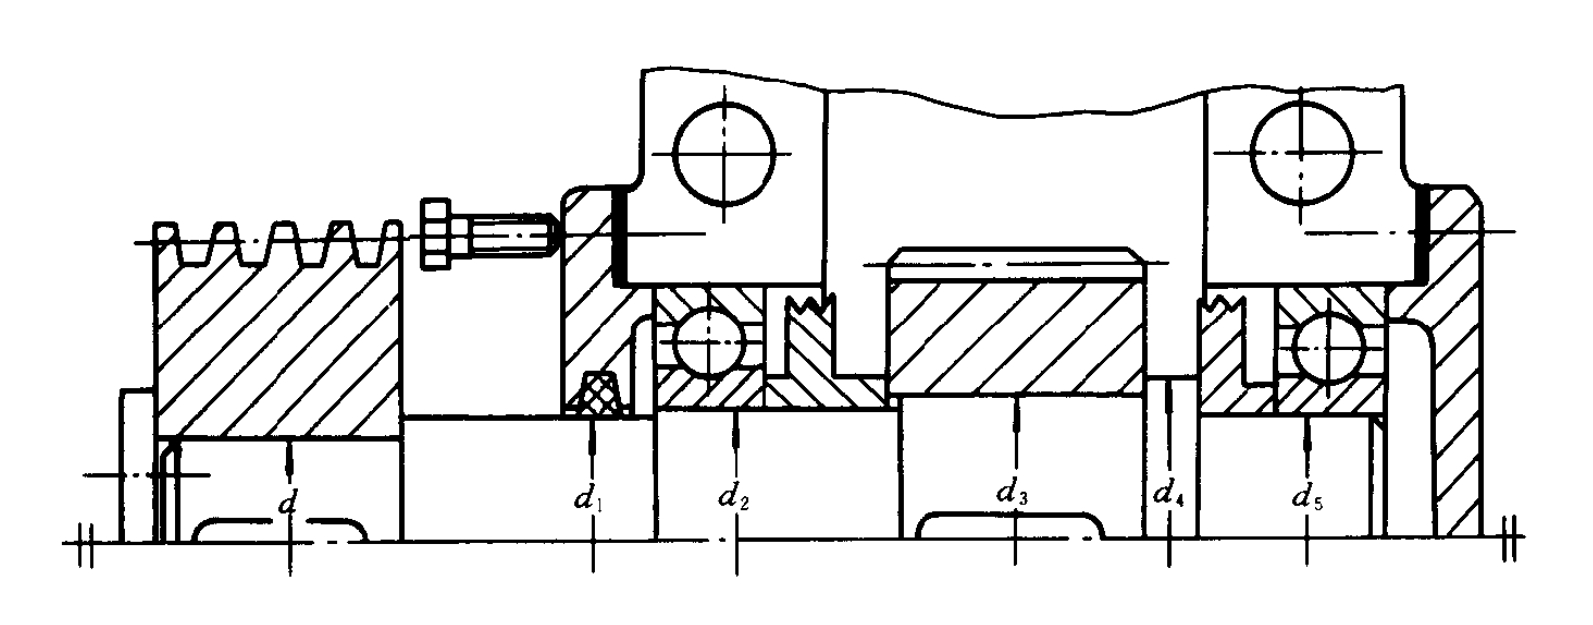
\includegraphics[scale = 0.2]{[2]P26 roller.png}
    \caption{脂润滑轴段设计参考}\label{figure9}
\end{figure}

\begin{enumerate}
    \item 优先确定 $d_3$ 处的轴段,因其右端与齿轮轮毂齐平,左端只需要根据大齿轮轮毂宽减去 $1\sim 2\text{mm}$即可;
    \item 接下来可以确定 $d_5$ 处轴段长,其右端与轴承端面齐平,左端与封油盘齐平,封油盘参数见 [2]P30 图 4-10;
    \item 在$d_3$左端确定好定位之后,$d_2$的轴段长度也已经确定;
    \item 再确定$d$的轴段长,该轴段长根据轴伸配合的带轮或联轴器的轮毂长度确定,在之前的“带轮的选择”与“联轴器的选择”两节中已确定;
    \item 现剩下$d_1$长度无法确定,该轴段需要留出一个$Md_3$螺钉的距离,以便在不拆下带轮的情况下,拆卸轴承端盖,因此,需要在轴承端盖凸缘外再加一个$Md_3$螺栓长度与一定余量($5\sim 8$mm),螺栓长度可根据下式计算:
    $$L = k + e + (1.25\sim 1.5)d_3$$
    其中,$e$为轴承端盖厚度,$k$为螺帽厚度,$d_3$为螺栓公称直径,可由 [2]P130 表 13-7 查得。
\end{enumerate}

\subsection{键的选择}

本项目中高低速轴与齿轮轮毂连接处选用 A 型平键作为键连接方式,轴伸与带轮、联轴器连接处选用 C 型平键作为键连接方式,根据轴的直径,查 [2]P140 表 14-1 可得键的型号见表\ref{table16}所示。

\begin{table}[htbp]
    \centering
    \setlength{\belowcaptionskip}{0.3cm}
    \caption{各个轴段选取的键连接型号}
    \begin{tabular}{c c c c}
        \toprule
        轴段 & 键的类型 & 键的公称尺寸  & 键长/mm \\
        \midrule
        高速轴与齿轮轮毂连接   & A 型 & $14\times 9$    & 110\\
        低速轴与齿轮轮毂连接   & A 型 & $20\times 12$   & 90\\
        高速轴与带轮连接      & C 型  & $10\times 8$     & 56\\
        低速轴与联轴器连接    & C 型  &  $14 \times 9$    & 70\\
        \bottomrule
    \end{tabular}
    \label{table16}
\end{table}

\section{减速器箱体设计}
\subsection{铸铁减速器箱体结构尺寸}

查阅 [2]P17 表 3-1 对减速器的箱体结构尺寸进行设计,其中螺纹直径查 [2]P126 表 13-1,并且统一两轴承端盖尺寸,计算出发现高速轴与低速轴所需轴承盖尺寸不同,统一换为较大者,表格为调整后结果。

\begin{table}[htbp]
    \centering
    \setlength{\belowcaptionskip}{0.3cm}
    \caption{减速器箱体结构设计尺寸}
    \begin{tabular}{c c l c}
        \toprule
        \textbf{名称} & \textbf{符号} & \textbf{尺寸计算公式} & \textbf{设计尺寸/mm} \\
        \midrule
        箱座壁厚                      & $\delta$    & $\delta = max\{0.025a+1,8\}$    & 8 \\
        箱盖壁厚                      & $\delta_1$  & $\delta_1 = max\{0.02a+1,8\}$   & 8 \\
        \multirow{3}{*}{箱体凸缘厚度} & 箱座$b$      & $b=1.5\delta $                  & 12\\
                                     & 箱盖$b_1$    & $b_1 =1.5\delta_1$              & 12\\
                                     & 箱底座$b_2$  & $b_2 =2.5\delta$                & 20 \\
        \multirow{2}{*}{加强肋厚}     & 箱座$m$      & $m=0.85\delta $                & 7 \\
                                     & 箱盖$m_1$    & $m_1=0.85\delta_1$              & 7\\
        地脚螺钉直径                  & $d_f$        & $d_f=0.036a+12$                 & 20 \\
        轴承旁联接螺栓直径             & $d_1$        & $d_1=0.75d_f$                  & 18\\
        箱盖、箱座联接螺栓直径         & $d_2$        & $d_2=(0.5\sim 0.6)d_f$         & 12 \\
        轴承盖螺钉直径                & $d_3$        & \multirow{2}{*}{查 [2]P77 表 9-9} & 10 \\
        轴承盖螺钉数目                & $n$          &                   & 6\\
        轴承盖(轴承座端面)外径       & $D_2$        & $D_2=D+5d_3$                    & 190 \\
        轴承两侧联接螺栓间距离         & $s$          & $s\approx D_2$                  & 190\\
        观察孔盖螺钉直径              & $d_4$        & $d_2=(0.3\sim 0.4)d_f$          & 8 \\
        $d_f$至箱外壁距离             & $C_{1,min}$  & \multirow{6}{*}{查 [2]P17 表 3-1}  & 30\\
        $d_f$至凸缘外缘距离           & $C_{2,min}$  & & 26\\
        $d_1$至箱外壁距离             & $C_{1,min}$  & & 24\\
        $d_1$至凸缘外缘距离           & $C_{2,min}$  & & 22\\
        $d_2$至箱外壁距离             & $C_{1,min}$  & & 18\\
        $d_2$至凸缘外缘距离           & $C_{2,min}$  & & 16\\

         \bottomrule
    \end{tabular}
    
    \label{table11}
\end{table}

\subsection{减速器零件的位置尺寸}

接下来根据 [2]P24 表 4-1 对减速器零件的位置尺寸进行确定,经过计算后得到的结果如表\ref{table30}所示。

\begin{table}[htbp]
    \centering
    \setlength{\belowcaptionskip}{0.3cm}
    \caption{减速器零件的位置设计尺寸}
    \begin{tabular}{c c c c}
        \toprule
        名称 & 符号 & 设计尺寸/mm \\
        \midrule
        齿轮顶圆至箱体内壁的距离     & $\Delta_1$ & 10 \\
        齿轮端面至箱体内壁的距离     & $\Delta_2$ & 10 \\
        轴承端面至箱体内壁的距离     & $\Delta_3$ & 11 \\
        齿轮顶圆至轴表面距离         & $\Delta_5$ & 12 \\
        大齿轮齿顶圆至箱体内壁的距离  & $\Delta_6$ & 42 \\
        箱底至箱底内壁的距离         & $\Delta_7$ & 20 \\
        减速器中心高                & $H$        & 240 \\
        箱体内壁至轴承座孔端面的距离  & $L_1$      & 60 \\
        轴承端盖凸缘厚度            & $e$         & 12(轴 2)\\
        
        \bottomrule
    \end{tabular}
    
    \label{table30}
\end{table}





\section{键的校核}

键的材料采用强度极限$\sigma_B\ge 600\text{MPa}$的碳钢,通常用 45 钢,根据 [1]P163 表 10-11 查得,连接键挤压许用应力$[\sigma_p]=125\sim 150\text{MPa}$,键的截面尺寸按轴径选取后如表\ref{table16}所示,接下来对键进行强度校核。


\subsection{高速轴与齿轮轮毂连接键}

$$\sigma_p=\frac{4T}{dhl}=\frac{4\times 219198}{50\times 9\times 96}=20.29\text{MPa}\le 125\text{MPa}$$

\subsection{低速轴与齿轮轮毂连接键}

$$\sigma_p=\frac{4T}{dhl}=\frac{4\times 643917}{67\times 12\times 70}=45.76\text{MPa}\le 125\text{MPa}$$

\subsection{高速轴与带轮连接键}

$$\sigma_p=\frac{4T}{dhl}=\frac{4\times 223672}{35\times 8\times 46}=69.46\text{MPa}\le 125\text{MPa}$$

\subsection{低速轴与联轴器连接键}

$$\sigma_p=\frac{4T}{dhl}=\frac{4\times 643917}{50\times 9\times 56}=102.20\text{MPa}\le 125\text{MPa}$$

综上所述,各连接键均能通过校核。

\section{轴的校核}

\subsection{高速轴的校核}
\subsubsection{齿轮径向力与圆周力的计算}

取载荷系数 $K_d=1.2$,依据 [1]P173 式 (11-1),可得圆周力与径向力:

$$F_t=K_d\frac{2T_1}{d_1}=1.2\times \frac{2\times 219198.6}{116}=4535.16\text{N}$$

$$F_r=F_t\tan{\alpha} = 4535.16\times \tan(20)=1650.7\text{N}$$

\subsubsection{带压轴力的计算}

由带轮设计计算中可以得到,带的压轴力为:

$$F = 2zF_0\sin \frac{\alpha_1}{2}=2100.38\text{N}$$

\subsubsection{高速轴的校核}

已知作用在齿轮上的圆周力$F_t=4535.16\text{N}$,径向力为$F_r=1650.7\text{N}$,小齿轮分度圆直径$d_1=116\text{mm}$,作用在轴左端带轮上的外力$F=2100.38\text{N}$(方向未定),$L=192\text{mm}, K=124.5\text{mm}$(如图\ref{figure10}(a) 所示)。

(1)求垂直面的支承力(如图\ref{figure10}(b) 所示)

$$F_{1V}=\frac{F_r\frac{L}{2}}{L}=\frac{F_r}{2}=825.3\text{N}$$

$$F_{2V}=F_r-F_{1v}=825.3\text{N}$$

(2)求水平面的支承力(如图\ref{figure10}(c) 所示)

$$F_{1H}=F_{2H}=\frac{F_t}{2}=\frac{4535.16}{2}\text{N}=2267.6\text{N}$$

(3)$F$在支点产生反力(如图\ref{figure10}(d) 所示)

$$F_{2F}=\frac{FK}{L}=\frac{2100.38\times 124.5}{192}=1361.97\text{N}$$

$$F_{1F}=F+F_{1F}=3462.35\text{N}$$

外力$F$作用方向与带传动的布置有关,在具体布置尚未确定之前,可按照最不利的情况考虑。

(4)绘制垂直面的弯矩图(如图\ref{figure10}(b) 所示)

$$M_{aV}=F_{1V}\frac{L}{2}=79.23\text{N·m}$$

(5)绘制水平面的弯矩图(如图\ref{figure10}(c) 所示)

$$M_{aH}=F_{1H}\frac{L}{2}=217.69\text{N·m}$$

(6)$F$力产生的弯矩图(如图\ref{figure10}(d) 所示)

$$M_{1F}=FK=261.49\text{N·m}$$

$a-a$平面处$F$产生的弯矩为

$$M_{aF}=F_{2F}\frac{L}{2}=332.39\text{N·m}$$

(7)求合成弯矩图(如图\ref{figure10}(e) 所示)

考虑最不利情况,将$M_{aF}$与$\sqrt{M_{aH}^2+M_{aV}^2}$直接相加求和,则:

\begin{align*}
    M_a  & = \sqrt{M_{aV}^2+M_{aH}^2}+M_{aF}\\
         & = (\sqrt{79.23^2+217.69^2}+332.39)\text{N·m}\\
         & = 564.05\text{N·m}
\end{align*}

(8)求轴传递的转矩(如图\ref{figure10}(f) 所示)

$$T=F_t\frac{d_1}{2}=4535.16\times \frac{0.116}{2}=263.03\text{N·m}$$

(9)求危险截面的当量弯矩

易从图\ref{figure10}(g) 中看出,$a-a$截面最危险,其当量弯矩为
$$M_e=\sqrt{M_a^2+(\alpha T)^2}$$
如认为轴的扭切应力是脉动循环变应力,取折合系数$\alpha=0.6$,代入上式可得
$$M_e=\sqrt{564.05^2+(0.6\times 263.03)^2}\text{N·m}=585.71\text{N·m}$$

\begin{figure}[htbp]
    \centering
    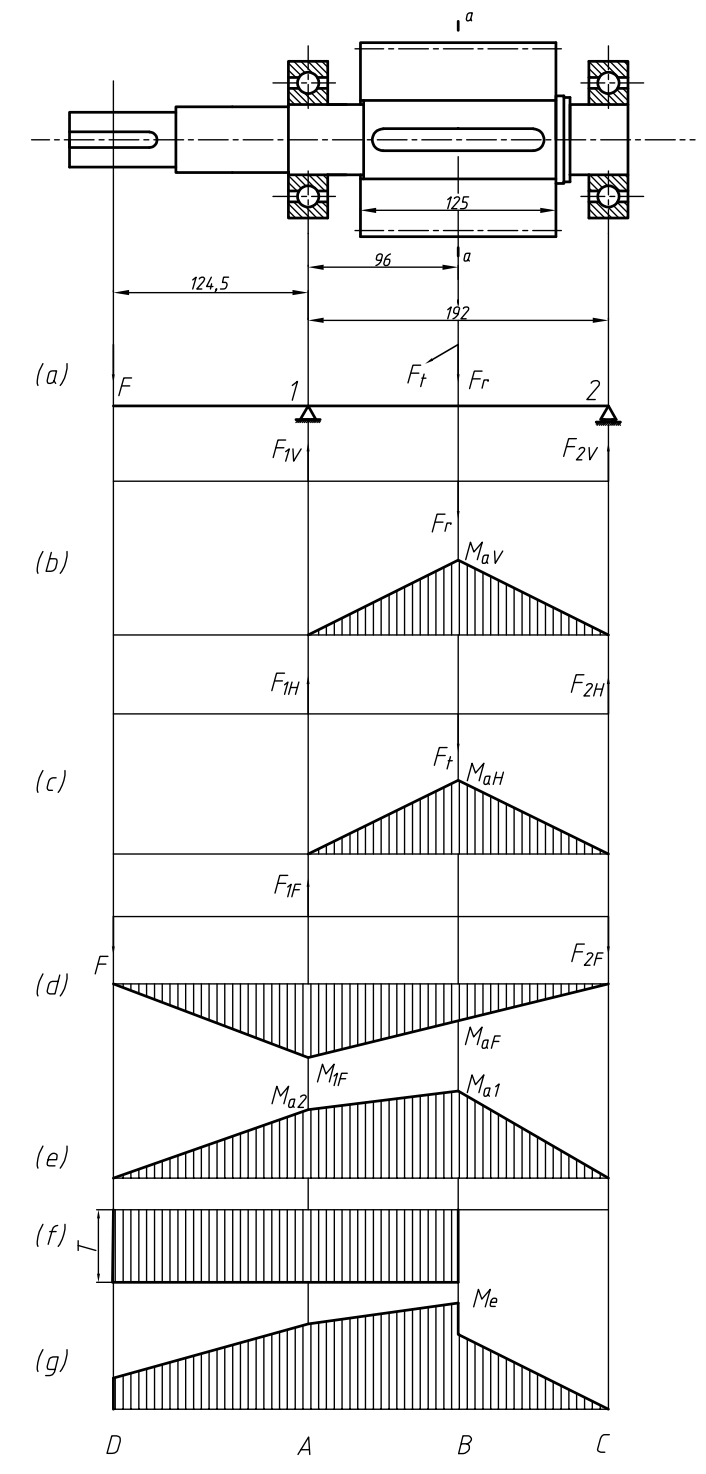
\includegraphics[scale = 0.4]{high_speed_roller.png}
    \caption{高速轴校核弯矩图}\label{figure10}
\end{figure}

(10)计算危险截面处轴的直径

轴的材料选用 45 钢,调质处理,由 [1]P246 表 14-1 查得$\sigma_B=650\text{MPa}$,由 [1]P251 表 14-3 查得 $[\sigma_{-1b}]=65\text{MPa}$,则有
$$d\ge \sqrt[3]{\frac{M_e}{0.1[\sigma_{-1b}]}}=\sqrt[3]{\frac{585.71\times 10^3}{0.1\times 65}}\text{mm}=44.83\text{mm}$$
考虑键槽对轴的削弱,将$d$值加大 5\%,故:
$$d=1.05\times 44.83\text{mm}=47.07\text{mm}$$

在本设计中,$a-a$截面的轴径设计为$50\text{mm}\ge 47.07\text{mm}$,故高速轴通过校核检验。

(11)其余轴段直径校核

如图\ref{figure10}所示定义$A,B,C,D$四个截面,其中$a-a$与$B$平面一致,步骤(10)中已校核。对$A$平面,
$$M_A=\sqrt{M_{AV}^2+M_{AH}^2}+M_{1F}=261.49\text{N·m}$$
$$M_{Ae}=\sqrt{M_A^2+(\alpha T)^2}=\sqrt{261.49^2+(0.6\times 263.03)^2}\text{N·m}=305.42\text{N·m}$$
$$d_A\ge \sqrt[3]{\frac{M_{Ae}}{0.1[\sigma_{-1b}]}}=\sqrt[3]{\frac{305.42\times 10^3}{0.1\times 65}}=36.09\text{mm}$$
考虑键槽对轴的削弱,将$d$值加大 5\%,故:
$$d=1.05\times 36.09\text{mm}=37.88\text{mm}$$ 
此时$A$截面轴径设计为$45\text{mm}> 37.88\text{mm}$,符合设计要求。

对$C$平面,作用在轴上的弯矩为 0,故不需要校核。

对$D$平面,作用在轴上的弯矩为
$$M_{De}=\alpha T=157.82\text{N·m}$$
$$d_D \ge \sqrt[3]{\frac{M_{Ae}}{0.1[\sigma_{-1b}]}}=\sqrt[3]{\frac{157.82\times 10^3}{0.1\times 65}}=28.95\text{mm}$$
考虑键槽对轴的削弱,将$d$值加大 5\%,故:
$$d=1.05\times 28.95\text{mm}=30.40\text{mm}$$ 
此时$D$截面轴径设计为$35\text{mm}> 30.40\text{mm}$,符合设计要求,综上所述,高速轴通过校核,符合强度要求。

\subsubsection{低速轴的校核}

\subsubsection{齿轮径向力与圆周力的计算}

取载荷系数$K_d=1.2$,依据 [1]P173 式 (11-1),可得圆周力与径向力:

$$F_t=K_d\frac{2T_1}{d_1}=1.2\times \frac{2\times 643917.9}{356}=4341.01\text{N}$$

$$F_r=F_t\tan{\alpha} = 4341.01\times \tan(20)=1580.00\text{N}$$

\subsubsection{低速轴的校核}

已知作用在齿轮上的圆周力$F_t=4341.01\text{N}$,径向力为$F_r=1580.00\text{N}$,大齿轮分度圆直径$d_2=356\text{mm}$,$L=200\text{mm}, K=137\text{mm}$(如图\ref{figure10}(a) 所示)。


(1)求垂直面的支承力(如图\ref{figure11}(b) 所示)

$$F_{1V}=F_{2V}=\frac{F_r}{2}=\frac{1580}{2}\text{N}=790\text{N}$$

(2)求水平面的支承力(如图\ref{figure11}(c) 所示)

$$F_{1H}=F_{2H}=\frac{F_t}{2}=\frac{4341.01}{2}\text{N}=2170.51\text{N}$$

(3)绘制垂直面的弯矩图(如图\ref{figure11}(b) 所示)

$$M_{aV}=F_{1V}\frac{L}{2}=790\times \frac{0.200}{2}=79.00\text{N·m}$$

(4)绘制水平面的弯矩图(如图\ref{figure11}(c) 所示)

$$M_{aH}=F_{1H}\frac{L}{2}=2170.51\times \frac{0.200}{2}=217.01\text{N·m}$$

(5)求合成弯矩图(如图\ref{figure11}(d) 所示)

$$M_{a2}=\sqrt{M_{aV}^2+M_{aH}^2}=\sqrt{79.00^2+217.01^2}=230.94\text{N·m}$$

$$M_{a1}=\sqrt{M_{aV}^2+M_{aH}^2}=\sqrt{79.00^2+217.01^2}=230.94\text{N·m}$$

(6)求轴传递的扭矩图(如图\ref{figure11}(e) 所示)

$$T = F_t\frac{d_2}{2}=4341.01\times \frac{0.356}{2}=772.69\text{N·m}$$

(7)求危险截面的当量弯矩(如图\ref{figure11}(f) 所示)

能从图中看出,$a-a$截面为危险截面,其当量弯矩为
$$M_e=\sqrt{M_{a}^2+(\alpha T)^2}$$
认为轴的扭切应力是脉动循环变应力,取折合系数$\alpha =0.6$,代入上式可得
$$M_e=\sqrt{230.94^2+(0.6\times 772.69)^2}\text{N·m}=517.94\text{N·m}$$

(8)校核危险截面直径

由于轴的材料选择 45 钢,正火处理,由 [1]P246 表 14-1 查得$\sigma_B=600\text{MPa}$,由 [1]P251 表 14-3 查得 $[\sigma_{-1b}]=65\text{MPa}$,则危险截面的直径满足

$$d_a\ge \sqrt[3]{\frac{M_e}{0.1[\sigma_{-1b}]}}=\sqrt[3]{\frac{517.94\times 10^3}{0.1\times 65}}=43.03\text{mm}$$

由于键会对轴有削弱作用,需要将轴的直径提高 5\%,故

$$d_a=43.03\times 1.05=45.18\text{mm}$$

该处设计直径$67\text{mm}> 45.18\text{mm}$,故$a-a$截面校核通过。

(9)其余轴段直径校核

如图\ref{figure11}所示定义$A,B,C,D$四个截面,其中$a-a$与$A$平面一致,步骤(8)中已校核。对$C$平面,轴上的弯矩载荷为 0,故不需要载荷。

$D,B$平面,
$$M_{e1}=M_{e2}=\alpha T=0.6\times 772.69\text{N·m}=463.61\text{N·m}$$
则该平面上的直径满足
$$d_B\ge \sqrt[3]{\frac{M_{e1}}{0.1[\sigma_{-1b}]}} = \sqrt[3]{\frac{463.61\times 10^3}{0.1\times 65}}=41.47\text{mm}$$
由于键会对轴有削弱作用,需要将轴的直径提高 5\%,故
$$d_a=41.47\times 1.05=43.54\text{mm}$$
该处轴段设计直径为$50\text{mm}> 43.54\text{mm}$,故校核通过。
\begin{figure}[htbp]
    \centering
    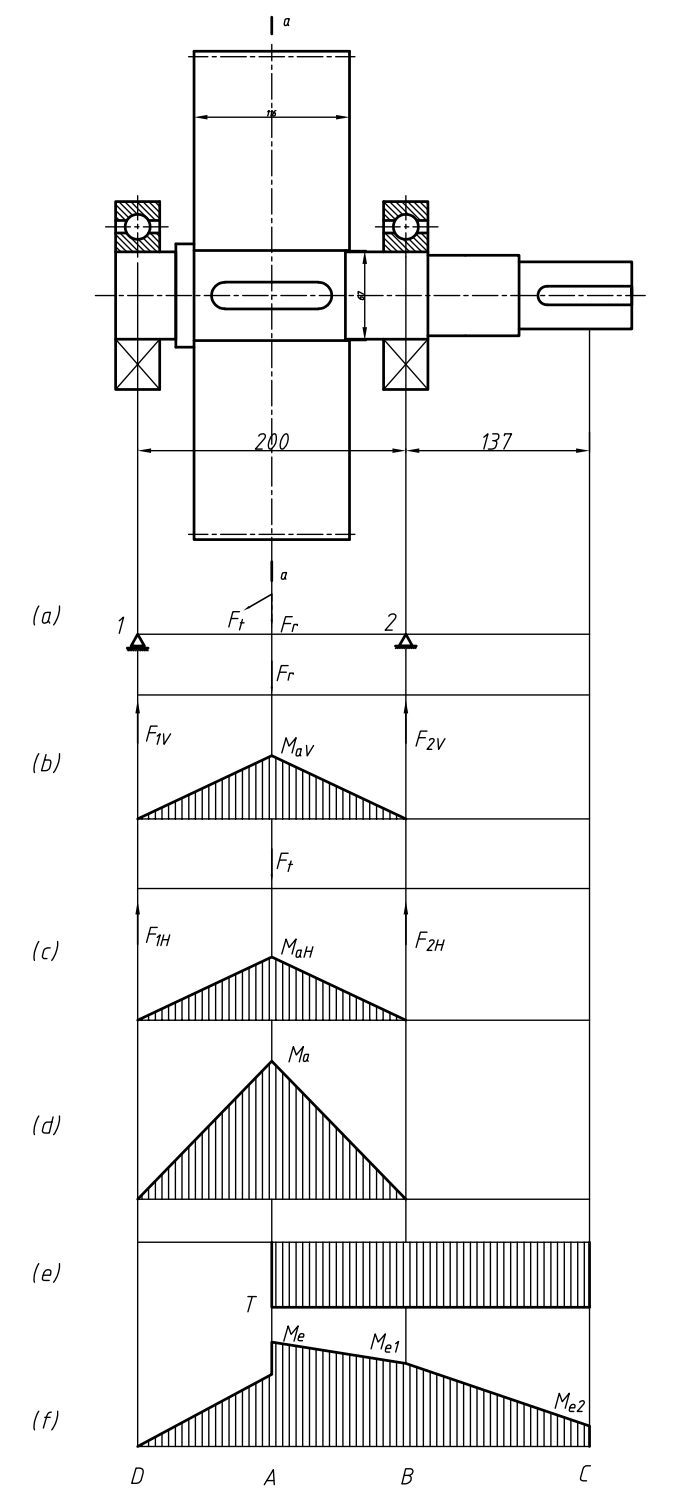
\includegraphics[scale = 0.4]{low_speed_roller.png}
    \caption{低速轴校核弯矩图}\label{figure11}
\end{figure}

\section{轴承的校核}

据题目要求,两班制工作,轴承每日工作时间为 16 小时,使用年限为 10 年,则轴承寿命要求为$L_0=16\times 365\times 10 \text{h}= 58400\text{h}$。


\subsection{高速轴轴承校核}

由于本设计中采取深沟球轴承,故深沟球轴承的当量载荷与其所受径向力相等,即$P=F_r$,深沟球轴承的各项参数如表\ref{table10}所示。由轴的校核可知,小齿轮径向力产生的垂直面的径向支承力:
$$F_{1V}=F_{2V}=\frac{F_r\frac{L}{2}}{L}=\frac{F_r}{2}=825.3\text{N}$$

小齿轮圆周力产生的水平面的径向支承力:
$$F_{1H}=F_{2H}=\frac{F_t}{2}=\frac{4535.16}{2}\text{N}=2267.6\text{N}$$

由带轮压轴力产生的垂直面内的径向支承力:
$$F_{2F}=\frac{FK}{L}=\frac{2100.38\times 124.5}{192}=1361.97\text{N}$$
$$F_{1F}=F+F_{2F}=3462.35\text{N}$$

则两轴承的径向合成力为:
\begin{align*}
    F_{r1} & =\sqrt{F_{1H}^2+(F_{1F}+F_{1V})^2}\\
        & = \sqrt{2267.6^2+(3462.35+825.3)^2}\text{N}\\
        & = 4850.36\text{N}\\
    F_{r2} & =\sqrt{F_{2H}^2+(F_{2V}-F_{2F})^2}\\
        & = \sqrt{2267.6^2+(825.3-1361.97)^2}\text{N}\\
        & = 2330.24\text{N}
\end{align*}


$$L_{1}=
\frac{10^6}{60n_1}\left(\frac{C_{r1}}{P_1}\right)^\varepsilon 
= \frac{10^6}{60\times 301}\left(\frac{40.8\times 10^3}{4850.36}\right)^3
=32956.5\text{h}<L_0$$

$$L_{2}=
\frac{10^6}{60n_2}\left(\frac{C_{r2}}{P_2}\right)^\varepsilon 
= \frac{10^6}{60\times 301}\left(\frac{40.8\times 10^3}{2330.24}\right)^3
=297208.14\text{h}>L_0$$

通过检验,发现 1 号轴承不满足寿命要求,需要更换,修正后的轴承见表\ref{table13},经过修正后,1 号轴承寿命为:
$$L_{1}=
\frac{10^6}{60n_1}\left(\frac{C_{r1}}{P_1}\right)^\varepsilon 
= \frac{10^6}{60\times 301}\left(\frac{59.5\times 10^3}{4850.36}\right)^3
=102214.20\text{h}>L_0$$

\subsection{低速轴轴承校核}

由轴的校核可知,大齿轮径向力产生的垂直面的径向支承力:
$$F_{1V}=F_{2V}=\frac{F_r}{2}=\frac{1580}{2}\text{N}=790\text{N}$$

大齿轮圆周力产生的水平面的径向支承力:
$$F_{1H}=F_{2H}=\frac{F_t}{2}=\frac{4341.01}{2}\text{N}=2170.51\text{N}$$

则两轴承的径向合成力为:
\begin{align*}
    F_{r1} =F_{r2}& =\sqrt{F_{1H}^2+F_{1V}^2}\\
        & = \sqrt{2170.51^2+790^2}\text{N}\\
        & = 2309.8\text{N}
\end{align*}

$$L_{1}=L_2=
\frac{10^6}{60n_1}\left(\frac{C_{r1}}{P_1}\right)^\varepsilon 
= \frac{10^6}{60\times 98}\left(\frac{72.2\times 10^3}{2309.8}\right)^3
=5194109\text{h}>L_0$$

由于此时轴承寿命超出题设工作寿命过多,可以考虑将轴承换成特轻直径系列轴承,经过调整后轴承参数如表\ref{table13}所示。
\begin{table}[htbp]
    \centering
    \setlength{\belowcaptionskip}{0.3cm}
    \caption{修正后轴承选用型号及参数}
    \begin{tabular}{c c c}
        \toprule
        型号及参数 & 高速轴 & 低速轴\\
        \midrule
        轴承型号 & 6409(新标准) & 6213(新标准) \\
        内径$d$/mm & 45 & 65 \\
        外径$D$/mm & 120 & 120 \\
        安装尺寸/mm & 55 & 74 \\
        轴承宽度/mm & 29 & 23 \\
        径向基本额定动载荷$C_r$/kN & 59.5 & 44.0 \\
        \bottomrule
    \end{tabular}
    
    \label{table13}
\end{table}

对轴承进行修正后,再次计算寿命可得:
$$L_{1}'=L_2'=
\frac{10^6}{60n_1}\left(\frac{C_{r1}}{P_1}\right)^\varepsilon 
= \frac{10^6}{60\times 98}\left(\frac{44.0\times 10^3}{2309.8}\right)^3
=1175594\text{h}>L_0$$
因此,低速轴轴承可通过校验。

\section{减速器附件设计}

\subsection{轴承盖(及套杯)的选择}

本设计采用凸缘式轴承盖,查 [2]P77 表 9-9,计算得到各参数如表\ref{table15}所示。

\begin{table}[hbp]
    \centering
    \setlength{\belowcaptionskip}{0.3cm}
    \caption{凸缘式轴承盖参数设计}
    \begin{tabular}{c l c c}
        \toprule
        参数名称 & 计算方法& 高速轴尺寸/mm & 低速轴尺寸/mm\\
        \midrule
        $D$   & 轴承外径     & 120  & 120 \\
        $d_0$ & $d_0=d_3+1$ & 11 & 11\\
        $D_0$ & $D_0=D + 2.5d_3$ & 145  & 145\\
        $D_2$ & $D_2=D_0 + 2.5d_3$ & 170 & 170 \\
        $e$   & $e=1.2d_3$        & 12 & 12  \\
        $D_4$ & $D_4=D-(10\sim 15)$ & 110 & 110 \\
        $D_5$ & $D_5=D_0-3d_3$    &  115 & 115\\
        \bottomrule
    \end{tabular}
    
    \label{table15}
\end{table}

\subsection{密封圈参数选择}

通过查表 [2] P158 表 16-9 可得,高速轴与低速轴的密封圈选择参数如下表\ref{table14}所示。


\begin{table}[hbp]
    
    
    \centering
    \setlength{\belowcaptionskip}{0.3cm}
    \caption{密封圈参数设计}
    \begin{tabular}{c l c c}
        \toprule
        参数名称 & 计算方法& 高速轴尺寸/mm & 低速轴尺寸/mm\\
        \midrule
        $d_0$   & 轴径     & 42  & 60 \\
        $d_1$   & 凸缘式轴承盖孔径 & 43 & 61\\
        $D_1$   & 密封圈外径 &  55 & 77\\
        $b_1$   & 密封圈外径宽 & 4  & 5 \\
        $b_2$   & 密封圈内径宽 & 5.5 & 7.1 \\ 
        \bottomrule
    \end{tabular}
    
    \label{table14}
\end{table}

\subsection{起重螺钉的选择}

查 [2]P80 表 9-21 可得起重螺栓的相关参数,本设计中取$M20$用作起重螺栓,计算可得相关参数如表\ref{table18}所示。
\begin{table}[htbp]
    \centering
    \setlength{\belowcaptionskip}{0.3cm}
    \caption{起重螺钉参数设计}

    \begin{tabular}{c c}
        \toprule
        参数名称    & 尺寸值/mm \\
        \midrule
        起重螺钉型号 &  AM16 GB2225-80\\
        $d$         &  M16\\
        $D$         &  35 \\
        $L$         &  62 \\
        $s$         &  27 \\
        $d_1$       &  16\\
        $l$         &  32 \\
        $l_1$       &  8  \\
        $l_2$       &  4  \\
        $l_3$       &  2  \\
        $C$         &  2 \\
        允许负荷     &  1.9kN \\
        $d_2$       &  22 \\
        $h$         &  6   \\
        $C_{1,min}$ &  22 \\
        $C_{2,min}$ &  20 \\
        \bottomrule
        注:$C_{1,min},C_{2,min}$为扳手空间。 &\\
    \end{tabular}
    
    \label{table18}
\end{table}

\subsection{窥视孔及视孔盖的选择}

本设计选用板结构视孔盖,查 [2]P80 表 9-18 可得其参数如表\ref{table19}所示。
\begin{table}[htbp]
    \centering
    \setlength{\belowcaptionskip}{0.3cm}
    \caption{板结构视孔盖参数设计}
    \begin{tabular}{c l c}
        \toprule
        参数名称  & 计算方法 & 尺寸值/mm \\
        \midrule
        $A$   &  -       &100\\
        $d_4$ &  螺栓直径 &8 \\
        $A_1$ &  $A_1 = A+(5\sim 6)d_4$ &140 \\
        $A_0$ & $A_0=0.5(A+A_1)$       & 120\\
        $B_1$ & $B_1=\text{箱体宽度}-(15\sim 20)$ & 142 \\
        $B$  & $B=B_1-(5\sim 6)d_4$    & 102\\
        $B_0$& $B_0=0.5(B+B_1)$        & 122\\
        $h$  & 铸铁选用 5              & 5 \\
        \bottomrule
    \end{tabular}
    
    \label{table19}
\end{table}

\subsection{通气螺塞的选择}

本设计选用无过滤装置的通气螺塞,查 [2]P76 表 9-6 可得其参数如表\ref{table20}所示。

\begin{table}[htbp]
    \centering
    \setlength{\belowcaptionskip}{0.3cm}
    \caption{通气螺塞参数设计}
    \begin{tabular}{c l c}
        \toprule
        参数名称  &  尺寸值/mm \\
        \midrule
        $d$      &  $M16\times 1.5$ \\
        $D$      &  22 \\
        $D_1$    &  19.6 \\
        $S$      &  17 \\
        $L$      &  23 \\
        $l$      &  12 \\
        $a$      &  2  \\
        $d_1$    &  5 \\
        \bottomrule
    \end{tabular}
    
    \label{table20}
\end{table}


\subsection{油面指示器的选择}
本设计选用压配式圆形油标,查 [2]P78 表 9-12 可得其参数如表\ref{table21}所示。
\begin{table}[htbp]
    \centering
    \setlength{\belowcaptionskip}{0.3cm}
    \caption{油面指示器参数设计}
    \begin{tabular}{c c}
        \toprule
        参数名称  &  尺寸值/mm \\
        \midrule
        型号     & 油标 A32GB1160.1-89\\
        $d$ & 32\\
        $D$ & 48\\
        $d_1$ & 35\\
        $d_3$ & 45 \\
        $H$ & 18\\
        O 型密封圈 & $38.7\times 3.55$\\
        \bottomrule
    \end{tabular}
    
    \label{table21}
\end{table}

\subsection{油塞的选择}
本设计选用外六角油塞,查 [2]P79 表 9-16 可得其参数如表\ref{table22}所示。
\begin{table}[htbp]
    \centering
    \setlength{\belowcaptionskip}{0.3cm}
    \caption{油塞参数设计}
    \begin{tabular}{c c}
        \toprule
        参数名称  &  尺寸值/mm \\
        \midrule
        $d$ & $M16\times 1.5$\\
        $D_0$ & 26\\
        $e$  & 19.6\\
        $L$ & 23\\
        $l$ & 12\\
        $a$ & 3\\
        $S$ & 17\\
        $d_1$ & 17\\
        $H $ & 2\\
        \bottomrule
    \end{tabular}
    
    \label{table22}
\end{table}

\subsection{起吊装置的选择}

起吊装置可通过查 [2] P80 表 9-20 得到,见表\ref{table24},\ref{table25},\ref{table26}所示。

\begin{table}[htbp]
    \centering
    \setlength{\belowcaptionskip}{0.3cm}
    \caption{箱盖吊耳参数设计}
    \begin{tabular}{c c c}
        \toprule
        参数名称  &  计算方法  & 尺寸值/mm \\
        \midrule
        $d$   & $d=(1.8\sim 2.5)\delta_1$ & 20 \\\
        $R$    &  $R=(1\sim 1.2)d$ & 20\\
        $e$    &  $R=(0.8\sim 1)d$ & 16\\
        $b$  & $b=2\delta_1$ & 16\\ 
        \bottomrule
    \end{tabular}
    
    \label{table24}
\end{table}

\begin{table}[htbp]
    \centering

    \setlength{\belowcaptionskip}{0.3cm}
    \caption{高速轴左侧箱座吊耳参数设计}
    \begin{tabular}{c c c}
        \toprule
        参数名称  &  计算方法  & 尺寸值/mm \\
        \midrule
        $B$  & $B=C_1+C_2$ & 47\\
        $H$  & $H=0.8B$  & 40\\
        $h$  & $h=0.5 H$ & 20 \\
        $r_2$ & $r_2=0.25B$ & 12 \\
        $b$ & $b=2\delta$ & 16\\
        \bottomrule
    \end{tabular}
    
    \label{table25}
\end{table}

\begin{table}[htbp]
    \centering
    \setlength{\belowcaptionskip}{0.3cm}
    \caption{低速轴右侧箱座吊耳参数设计}
    \begin{tabular}{c c c}
        \toprule
        参数名称  &  计算方法  & 尺寸值/mm \\
        \midrule
        $B$  & $B=C_1+C_2$ & 34\\
        $H$  & $H=0.8B$  & 28\\
        $h$  & $h=0.5 H$ & 14 \\
        $r_2$ & $r_2=0.25B$ & 10 \\
        $b$ & $b=2\delta$ & 16\\
        \bottomrule
    \end{tabular}
    
    \label{table26}
\end{table}


\subsection{各螺栓标准件选择}

各螺栓标准件的选择如表\ref{table23}所示。

\begin{table}[htbp]
    \centering
    \setlength{\belowcaptionskip}{0.3cm}
    \caption{螺栓与圆锥销国标型号}
    \begin{tabular}{l l}
        \toprule
        螺栓  &  国标 \\
        \midrule
        
        $Md_1$六角形螺栓 & GB5782-86 M20$\times $150  \\
        $Md_1$弹簧垫圈 & GB93-87 20\\
        $Md_1$螺母  & GB6170-86 M20\\
        $Md_2$六角形螺栓 & GB5783-86 M12$\times $45\\
        $Md_2$弹簧垫圈 & GB93-87 12\\
        $Md_2$螺母  & GB6170-86 M12\\
        $Md_3$六角形螺栓 & GB5783-86 M8$\times$20\\
        $Md_4$六角形螺栓 & GB5783-86 M10$\times$25\\
        销 & 销 GB117-86 A6$\times$28  \\
        \bottomrule
    \end{tabular}
    
    \label{table23}
\end{table}


\section{装配零件汇总表}
\begin{center}
\begin{longtable}{ccccc}
    \caption{装配零件代号、数量、材料汇总表}\label{table31}\\
    
    \toprule
    序号  &  代号  & 名称 &数量 &材料\\
    \midrule
    \endfirsthead
    \specialrule{0em}{0pt}{11.06pt}
    \multicolumn{5}{c}{续表\ref{table31}:装配零件代号、数量、材料汇总续表}\\
    \specialrule{0em}{0pt}{5.03pt}
    \toprule
    序号  &  代号  & 名称 &数量 &材料\\
    \midrule
    \endhead
    \bottomrule
    \endfoot

    1 & M12$\times$ 25         & 起盖螺钉 &1  & Q235\\
    2 &                        & 箱盖     &1  & HT200\\
    3 & GB5783-86 M8$\times$20 & 螺钉     &4  &Q235\\
    4 & M16$\times$1.5         & 通气螺塞 & 1 & Q235\\
    5 & GB5782-86 M20$\times$150&螺栓     & 6 & Q235\\
    6 & 垫圈 GB93-87 20        & 弹簧垫圈  &6  & 65Mn \\
    7 & GB6170-86 M20          & 螺母     & 6 & Q235 \\
    8 &                       & 视孔盖    & 1 & HT200\\
    9 &                       &垫片       & 1 &软钢纸板\\
    10 & 销 GB119-86 A6$\times $28& 圆锥销 & 2 &35\\
    11 & GB5783-86 M12$\times $ 45 & 螺栓  & 2 & Q235\\
    12 & 垫圈 GB93-87 12          & 弹簧垫圈 &2 & 65Mn\\
    13 & GB6170-86 M12           & 螺母     & 2 & Q235\\
    14 & A32GB1160.1-89          & 压配式圆形油标 & 1 & 组合件\\
    15 &                         & 封油垫   & 1 & 耐油橡胶、工业用革\\
    16 & M16 $\times $1.5         & 油塞    & 1 & Q235\\
    17 &                         & 轴承盖  & 1 & HT200\\
    18 &                         & 调整垫片 & 2 & 08F\\
    19 &                         & 封油盘   & 2 & Q235A\\
    20 & 键 C10$\times$56GB1096-79 & 键     & 1 & 45\\
    21 &                           & 低速轴     & 1 & 45\\
    22 & 毡圈 42FZ/T92010-91       & 毡圈   & 1 & 半粗羊毛毡\\
    23 &                          & 轴承盖  & 1 & HT200\\
    24 &                          & 调整垫片 & 2 & 08F\\
    25 & 键 20$\times$90 GB1096-79& 键      & 1 & 45\\
    26 & 6213 GB276-89            & 深沟球轴承 & 2 & \\
    27 &                          & 封油盘    & 2 & Q235A\\
    28 &                          & 大齿轮    & 1 & 45\\
    29 &                          & 箱座      & 2 & HT200\\
    30 &                          & 轴承盖    & 1 & HT200\\
    31 & 毡圈 60FZ/T92010-91      & 毡圈      & 1 & 半粗羊毛毡\\
    32 & 键 C14$\times$70GB1096-79& 键        & 1 & 45\\
    33 &                          & 高速轴        & 1 & 45\\  
    34 & GB5783-86 M10$\times$25  & 螺钉      & 24 & Q235\\
    35 & 6409 GB276-89            & 深沟球轴承& 2 & \\
    36 & 键 14$\times$110GB1096-79 & 键  & 1 & 45\\
    37 &                          & 轴承盖 & 1 & HT200\\
    38 &                          & 小齿轮 & 1 & 45\\

\end{longtable}
\end{center}
\newpage
\section{参考文献}

[1] 杨可桢,程光蕴。机械设计基础。6 版。北京:高等教育出版社,1979.

[2] 王昆。机械设计基础课程设计。北京:高等教育出版社,1995.

[3] 唐金松。简明机械设计手册。3 版。上海:上海科学技术出版社,1992.


\end{document}